Our proposal consists in two main components. First, to make the governance rules explicit, we propose to use a Domain Specific Language (DSL) including concrete constructs to define which decision rules must be followed to act on a set of tasks/patches. Secondly, we propose to enable the ``execution'' of the DSL specifications so that, beyond improving the understanding of the project internal organization, they can also be used to support and guide the collaboration among the project participants.

We believe our DSL would be useful in all the decision points identified before. Figure \ref{fig:process} illustrates how the application of our DSL would change the group dynamics in a particular decision point. As can be seen, given a set of tasks to be discussed in a decision point (i.e., either to accept them, accept a patch for them or include them in a release), users can vote for/against them (step 1), a decision engine analyzes the votes according to the governances rules defined (e.g., total agreement, simple majority, etc.) (step 2). As a result, the status of the tasks is changed based on the decisions taken by the engine (step 3). 

\begin{figure}[t]  
  \centering
  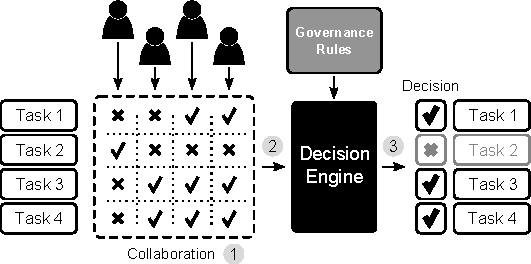
\includegraphics[width=0.6\textwidth]{./figures/processB}
  \caption{Decision process proposed.}
  \label{fig:process}
\end{figure}

In what follows we define the DSL and the infrastructure required to enable its use in practice in more detail.


